%Python code highlighting
\definecolor{mygreen}{rgb}{0,0.6,0}
\definecolor{mygray}{rgb}{0.5,0.5,0.5}
\definecolor{mymauve}{rgb}{0.58,0,0.82}

\lstset{ %
	backgroundcolor=\color{white},   % choose the background color; you must add \usepackage{color} or \usepackage{xcolor}; should come as last argument
	basicstyle=\footnotesize,        % the size of the fonts that are used for the code
	breakatwhitespace=false,         % sets if automatic breaks should only happen at whitespace
	breaklines=true,                 % sets automatic line breaking
	captionpos=b,                    % sets the caption-position to bottom
	commentstyle=\color{mygreen},    % comment style
	deletekeywords={...},            % if you want to delete keywords from the given language
	escapeinside={\%*}{*)},          % if you want to add LaTeX within your code
	extendedchars=true,              % lets you use non-ASCII characters; for 8-bits encodings only, does not work with UTF-8
	frame=single,	                   % adds a frame around the code
	keepspaces=true,                 % keeps spaces in text, useful for keeping indentation of code (possibly needs columns=flexible)
	keywordstyle=\color{blue},       % keyword style
	language=Octave,                 % the language of the code
	morekeywords={*,...},            % if you want to add more keywords to the set
	numbers=left,                    % where to put the line-numbers; possible values are (none, left, right)
	numbersep=5pt,                   % how far the line-numbers are from the code
	numberstyle=\tiny\color{mygray}, % the style that is used for the line-numbers
	rulecolor=\color{black},         % if not set, the frame-color may be changed on line-breaks within not-black text (e.g. comments (green here))
	showspaces=false,                % show spaces everywhere adding particular underscores; it overrides 'showstringspaces'
	showstringspaces=false,          % underline spaces within strings only
	showtabs=false,                  % show tabs within strings adding particular underscores
	stepnumber=2,                    % the step between two line-numbers. If it's 1, each line will be numbered
	stringstyle=\color{mymauve},     % string literal style
	tabsize=2,	                   % sets default tabsize to 2 spaces
	title=\lstname                   % show the filename of files included with \lstinputlisting; also try caption instead of title
}
\clearpage
\section{Fast Fourier Transform}
\begin{refsection}
\begin{tcolorbox}	
	\begin{tabular}{p{2.75cm} p{0.2cm} p{10.5cm}} 	
		\textbf{Header File}   &:& fft\_*.h \\
		\textbf{Source File}   &:& fft\_*.cpp \\
		\textbf{Version}       &:& 20180201 (Romil Patel)
	\end{tabular}
\end{tcolorbox}
%\subsubsection{Definitions of DFT and IDFT}
%The discrete Fourier transform of a sequence of N complex number $x_0, x_1, x_2,...,x_{N-1}$ into another sequance of complex number $X_0, X_1, X_2,...,X_{N-1}$ defined by,
%\begin{equation}
%X_k = \sum\limits_{n=0}^{N-1} x_n \cdot e^{-i2\pi kn/N}		\hspace{2cm}	0\leq k \leq N-1
%\end{equation}
%Similarly, inverse discrete Fourier transform can be given as,
%\begin{equation}
%x_n = \frac{1}{N} \sum\limits_{n=0}^{N-1} X_k \cdot e^{i2\pi kn/N}		\hspace{2cm}	0\leq k \leq N-1
%\end{equation}
%Using these equation, it requires $N^2$ calculation for the transformation from time domain to frequency domain and vice-versa. Therefore, it is not efficient for the practical implementation purpose. Radix-2 based FFT calculation reduces the number of computation to $Nlog n$.

\subsubsection{Algorithm}
The algorithm for the FFT will be implemented according with the following expression,
\begin{equation}
X_k =\dfrac{1}{\sqrt{N}}\sum\limits_{n=0}^{N-1} x_n \hspace{2mm} e^{i2\pi kn/N}		\hspace{2cm}	0\leq k \leq N-1
\label{FFT}
\end{equation}
Similarly, for IFFT,
\begin{equation}
x_n =\frac{1}{\sqrt{N}} \sum\limits_{k=0}^{N-1} X_k \hspace{2mm}  e^{-i2\pi kn/N}		\hspace{2cm}	0\leq k \leq N-1
\label{IFFT}
\end{equation}
From equations \ref{FFT} and \ref{IFFT}, we can write only one script for the implementations of the direct and inverse Discrete Fourier Transfer and manipulate its functionality as a FFT or IFFT by applying an appropriate input arguments. The generalized form for the algorithm can be given as,
\begin{equation}
y =\frac{1}{\sqrt{N}} \sum\limits_{n=0}^{N-1} x \hspace{2mm}  e^{m \hspace{1mm} i2\pi kn/N}		\hspace{2cm}	0\leq k \leq N-1
\label{FT}
\end{equation}
where, $x$ is an input complex signal, $y$ is the output complex signal and $m$ equals 1 or -1 for FFT and IFFT, respectively. An optimized fft function is also implemented without the $1/\sqrt(N) factor$, see below in the optimized fft section.

\subsubsection{Function description}
To perform FFT operation, the fft\_*.h header file must be included and the input argument to the function can be given as follows,
\begin{equation*}
y=f\hspace{-0.85mm}ft(x,1)
\end{equation*}
or
\begin{equation*}
	y = f\hspace{-0.85mm}ft(x)
\end{equation*}
where $x$ and $y$ are of the C++ type vector<complex>. In a similar way, IFFT can be manipulated as,
\begin{equation*}
x = f\hspace{-0.85mm}ft(y,1)
\end{equation*}
or
\begin{equation*}
	x = if\hspace{-0.85mm}ft(y)
\end{equation*}

\newpage
% Define block styles
\tikzstyle{decision} = [diamond, draw, fill=white!20,
text width=9em, text badly centered, node distance=3cm, inner sep=0pt]
\tikzstyle{block} = [rectangle, draw, fill=white!20,
text width=15em, text centered, rounded corners, minimum height=4em]
\tikzstyle{line} = [draw, -latex']
\tikzstyle{cloud} = [draw, ellipse,fill=white!20, node distance=3cm,
minimum height=3em]

\subsubsection{Flowchart}
The figure \ref{FFT_flowchart} displays top level architecture of the FFT algorithm.  If the length of the input signal is $2^N$, it'll execute Radix-2 algorithm otherwise it'll execute Bluestein algorithm \cite{Rao2010a}. The computational complexity of Radix-2 and Bluestein algorithm is $O(Nlog_{2}N)$, however, the computation of Bluestein algorithm involves the circular convolution which increases the number of computations. Therefore, to reduce the computational time it is advisable to work with the vectors of length $2^N$ \cite{Chu2000}.


\begin{figure}[h]
	\centering
	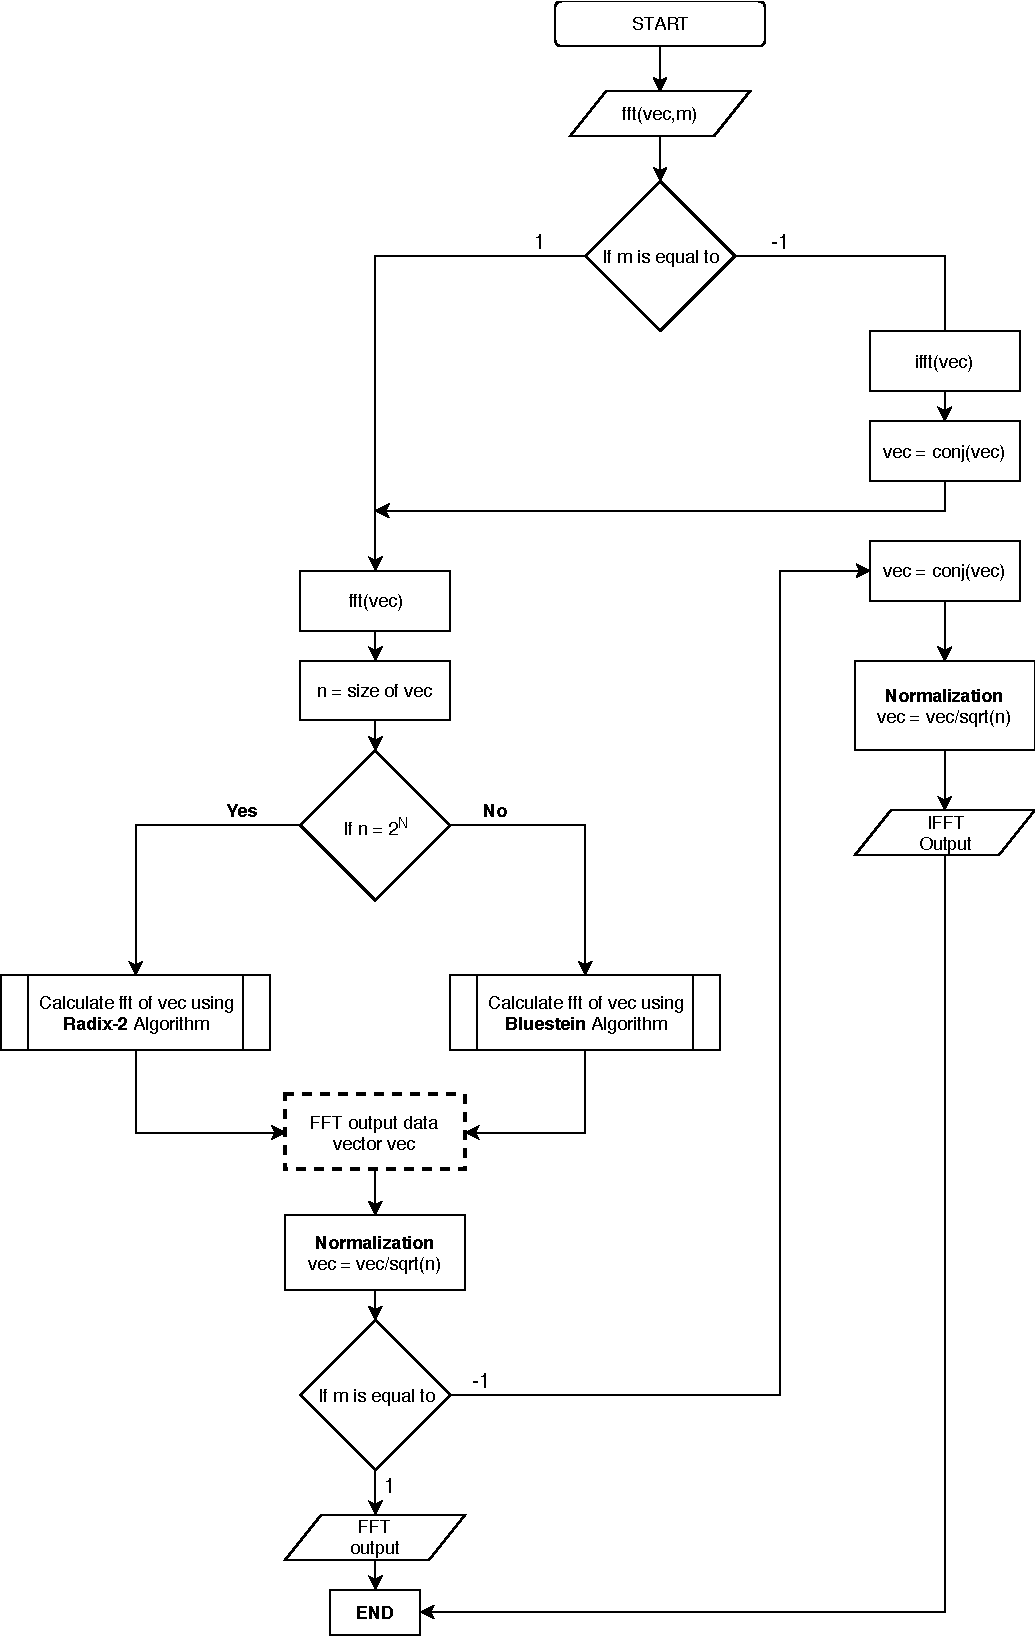
\includegraphics[width=10.5cm]{./algorithms/fft/figures/FFT_flowchart.pdf}
	\caption{Top level architecture of FFT algorithm}\label{FFT_flowchart}
\end{figure}



\newpage
\subsubsection{Radix-2 algorithm}
\begin{figure}[h]
	\centering
	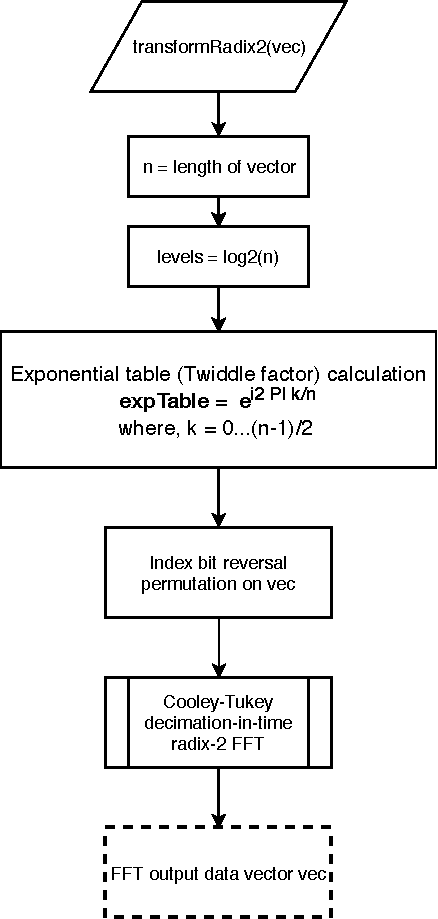
\includegraphics[width=6cm]{./algorithms/fft/figures/Radix2.pdf}
	\caption{Radix-2 algorithm}\label{Radix-2}
\end{figure}

\newpage
\subsubsection{Cooley-Tukey algorithm}
\begin{figure}[h]
	\centering
	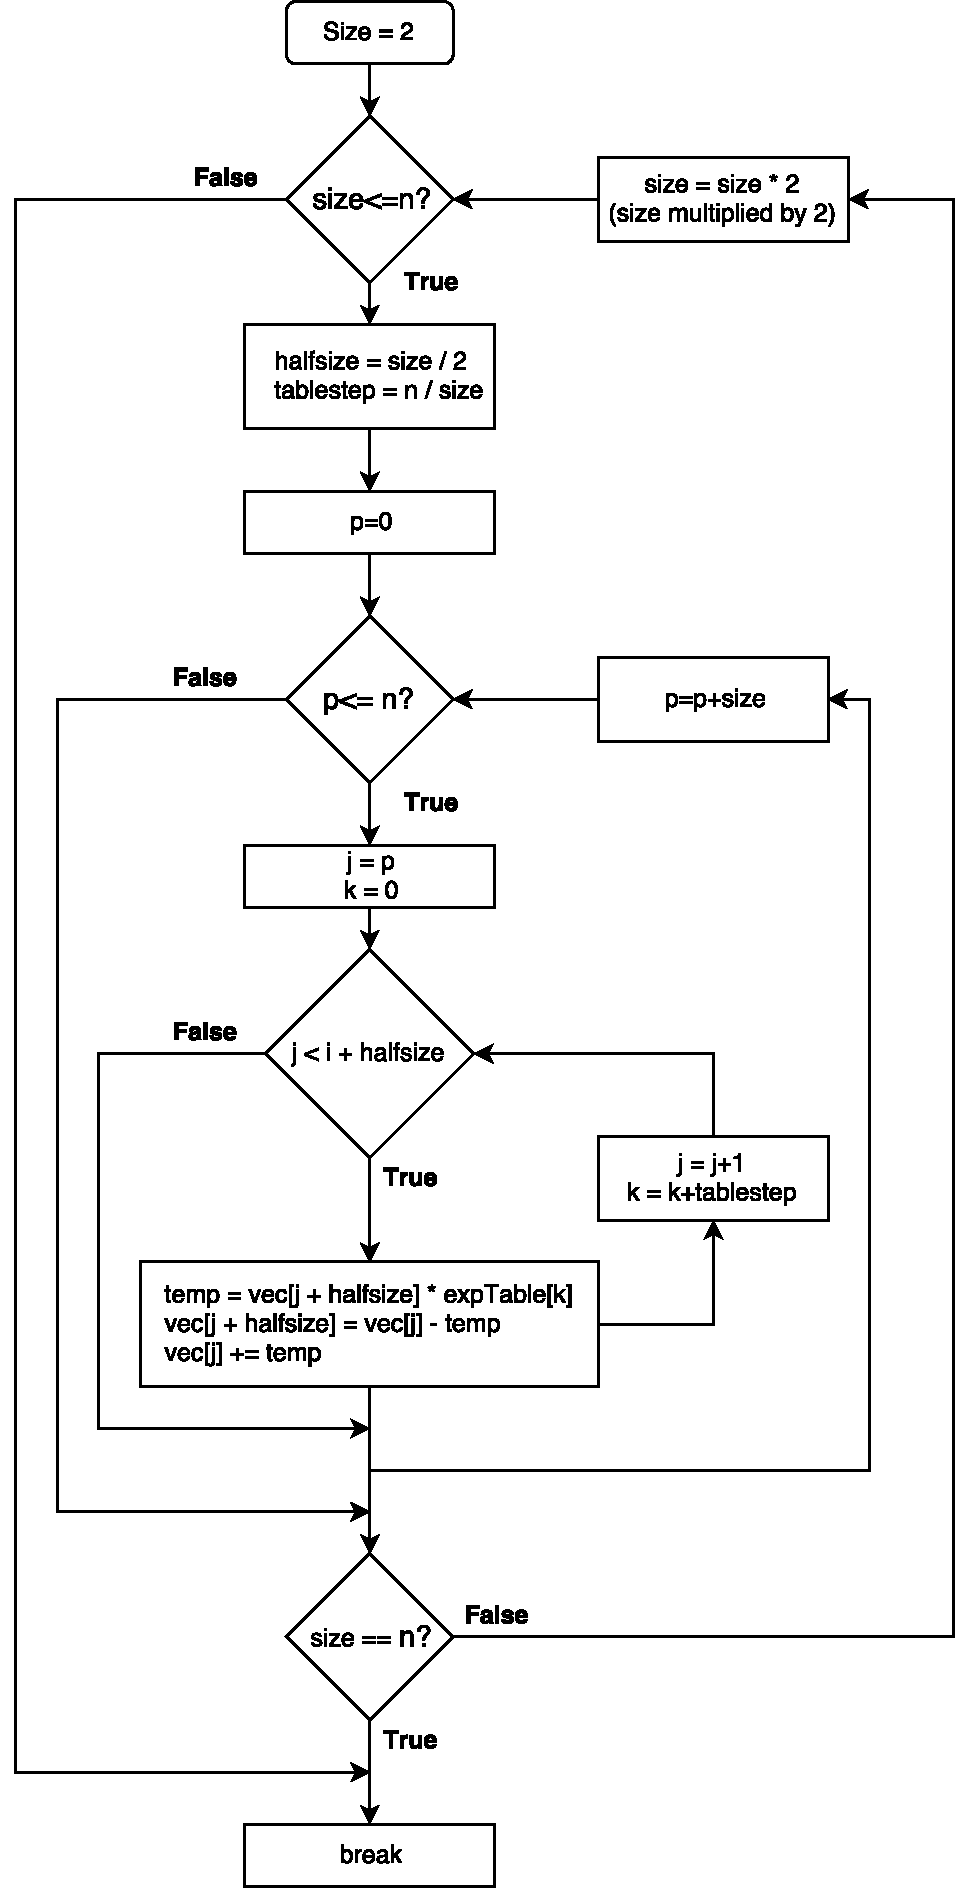
\includegraphics[width=10cm]{./algorithms/fft/figures/Cooley_Tukey.pdf}
	\caption{Cooley-Tukey algorithm}\label{Cooley_Tukey}
\end{figure}

\newpage
\subsubsection{Bluestein algorithm}
\begin{figure}[h]
	\centering
	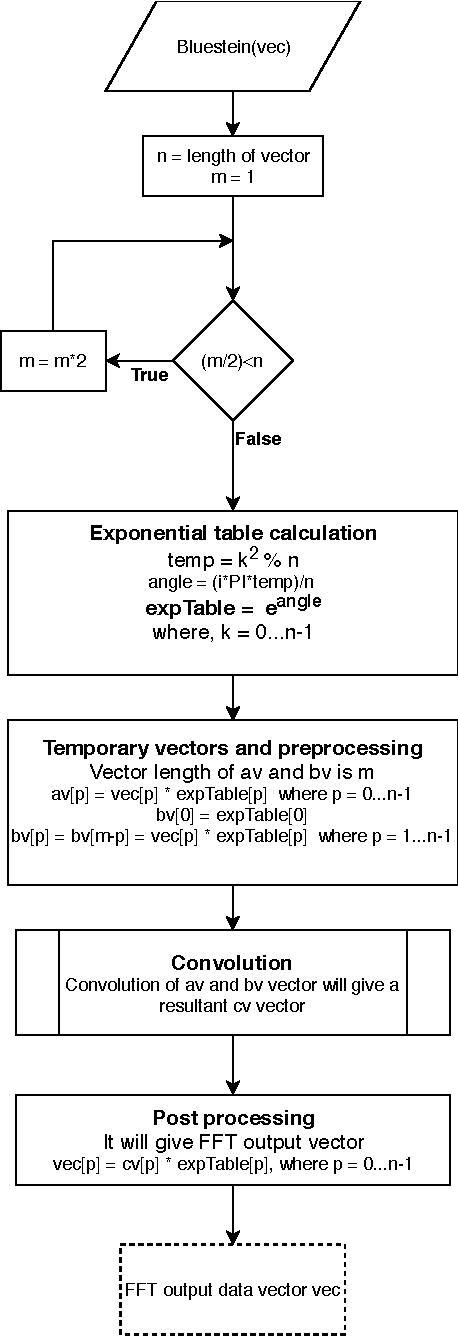
\includegraphics[width=6cm]{./algorithms/fft/figures/Bluestein.pdf}
	\caption{Bluestein algorithm}\label{Bluestein}
\end{figure}

\newpage
\subsubsection{Convolution algorithm}
\begin{figure}[h]
	\centering
	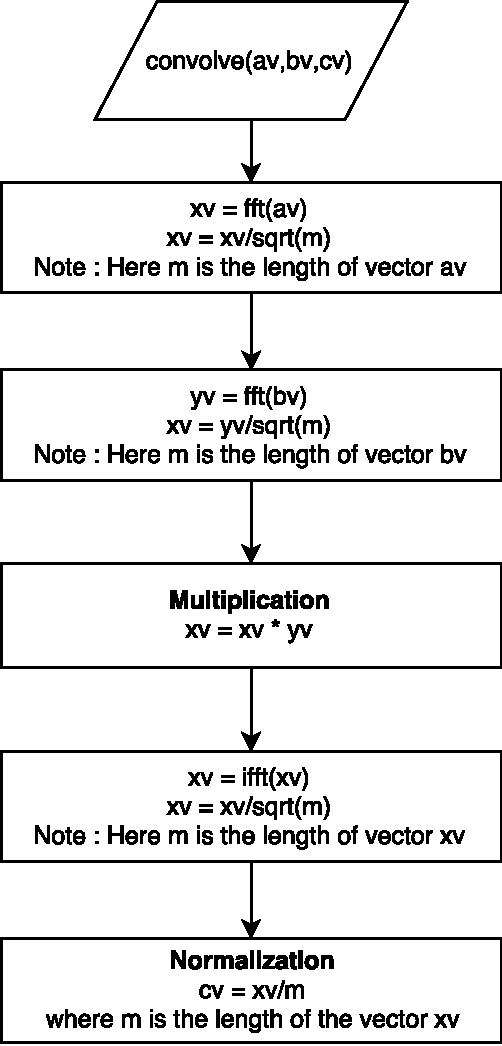
\includegraphics[width=6cm]{./algorithms/fft/figures/convolution.pdf}
	\caption{Circular convolution algorithm}\label{convolution}
\end{figure}





\newpage
\subsubsection{Test example}
This sections explains the steps to compare our C++ FFT program with the MATLAB FFT program.\\ \\
\textbf{Step 1} : Open the \textbf{fft\_test} folder by following the path "/algorithms/fft/fft\_test".\\ \\
\textbf{Step 2} : Find the \textbf{fft\_test.m} file and open it.\\
This fft\_test.m consists of two sections; section 1 generates the time domain signal and save it in the form of the text file with the name \textit{time\_function.txt} in the same folder. Section 2 reads the fft complex data generated by C++ program.\\
\lstinputlisting[language=Matlab, caption=fft\_test.m code]{../../algorithms/fft/fft_test/fft_test.m}
\textbf{Step 3} : Choose for sig a value between [1, 7] and run the first section namely \textbf{section 1} by pressing "ctrl+Enter".\\
This will generate a \textit{time\_function.txt} file in the same folder which contains the time domain signal data.\\ \\
\textbf{Step 4} : Now, find the \textbf{fft\_test.vcxproj} file in the same folder and open it.\\
In this project file, find \textit{fft\_test.cpp} and click on it. This file is an example of FFT calculation using C++ program. Basically this \textit{fft\_test.cpp} file consists of four sections:\\
\textbf{Section 1.} Read the input text file (import "time\_function.txt" data file)\\
\textbf{Section 2.} It calculates FFT.\\
\textbf{Section 3.} Save FFT calculated data (export \textit{frequency\_function.txt} data file).\\
\textbf{Section 4.}  Displays in the screen the FFT calculated data and length of the data.\\
\lstinputlisting[language=C++, caption=fft\_test.cpp code]{../../algorithms/fft/fft_test/fft_test.cpp}
\textbf{Step 5} : Run the \textit{fft\_test.cpp} file.\\
This will generate a \textit{frequency\_function.txt} file in the same folder which contains the Fourier transformed data.\\ \\
\textbf{Step 6} : Now, go to the \textbf{fft\_test.m} and run section 2 in the code by pressing "ctrl+Enter".\\
The section 2 reads \textit{frequency\_function.txt} and compares both C++ and MATLAB calculation of Fourier transformed data.

%The input signal applied to the C++ program must be a complex value vector. If your signal contains only real value then append 0 as an imaginary part in the vector of input signal.The Figure \ref{FFT_calculation_example}  displays one example of FFT calculation using C++ code in the simulator.

%\begin{figure}[h]
%	\centering
% \includegraphics[width=15cm]{./algorithms/fft/figures/ReIm2complex.jpg}
%	\caption{FFT calculation example}\label{FFT_calculation_example}
%\end{figure}

\subsubsection{Resultant analysis of various test signals}

The following section will display the comparative analysis of MATLAB and C++ FFT program to calculate several type of signals.

\subsubsection{1. Signal with two sinusoids and random noise}

\begin{figure}[h]
	\centering
	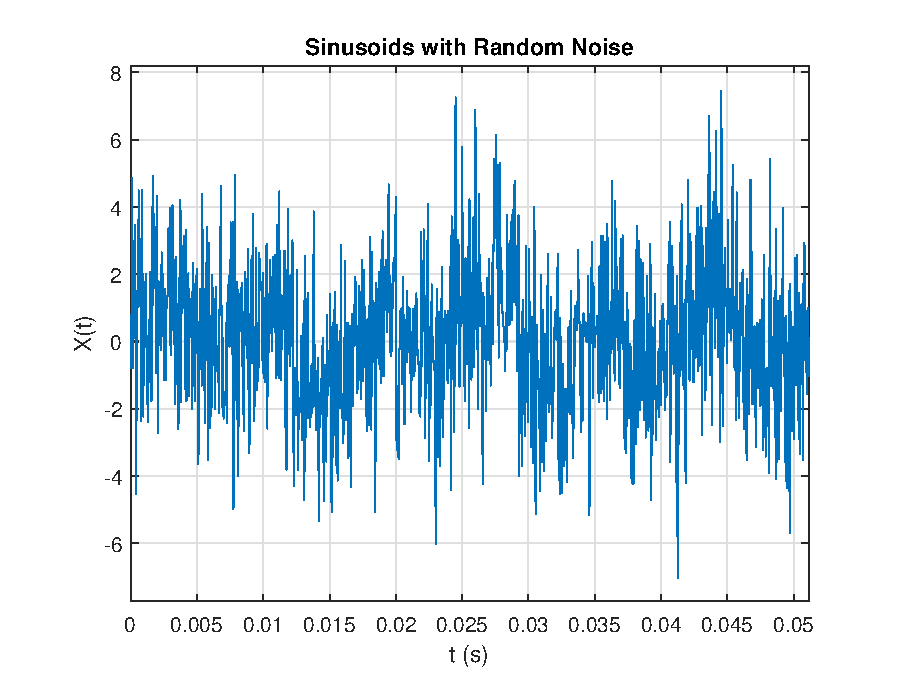
\includegraphics[width=12cm]{./algorithms/fft/figures/random_noise.eps}
	\caption{Random noise and two sinusoids}\label{random_noise}
\end{figure}

\begin{figure}[h]
	\centering
	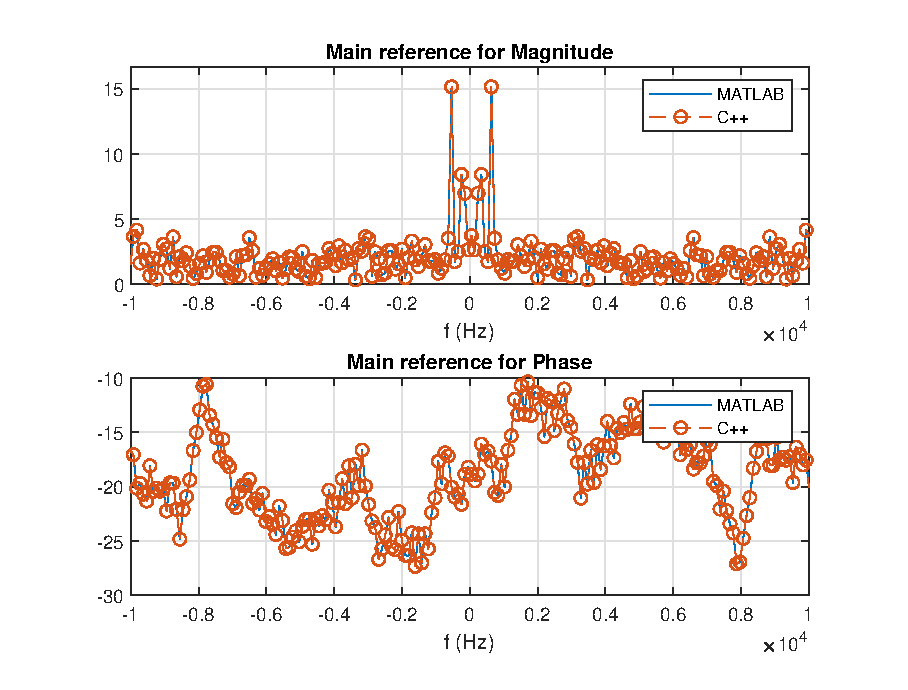
\includegraphics[width=12cm]{./algorithms/fft/figures/random_noise_fft.eps}
	\caption{MATLAB and C++ comparison}\label{random_noise_fft}
\end{figure}

\newpage
\subsubsection{2. Sinusoid with an exponent}

\begin{figure}[h]
	\centering
	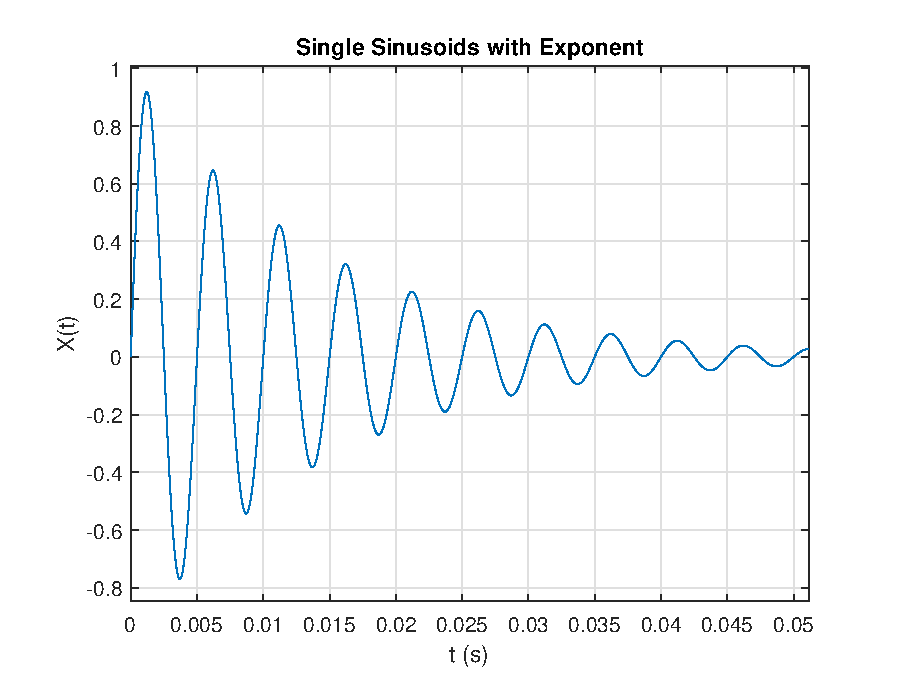
\includegraphics[width=12cm]{./algorithms/fft/figures/Single_sinusoid.eps}
	\caption{Sinusoids with exponent}\label{Single_sinusoid}
\end{figure}

\begin{figure}[h]
	\centering
	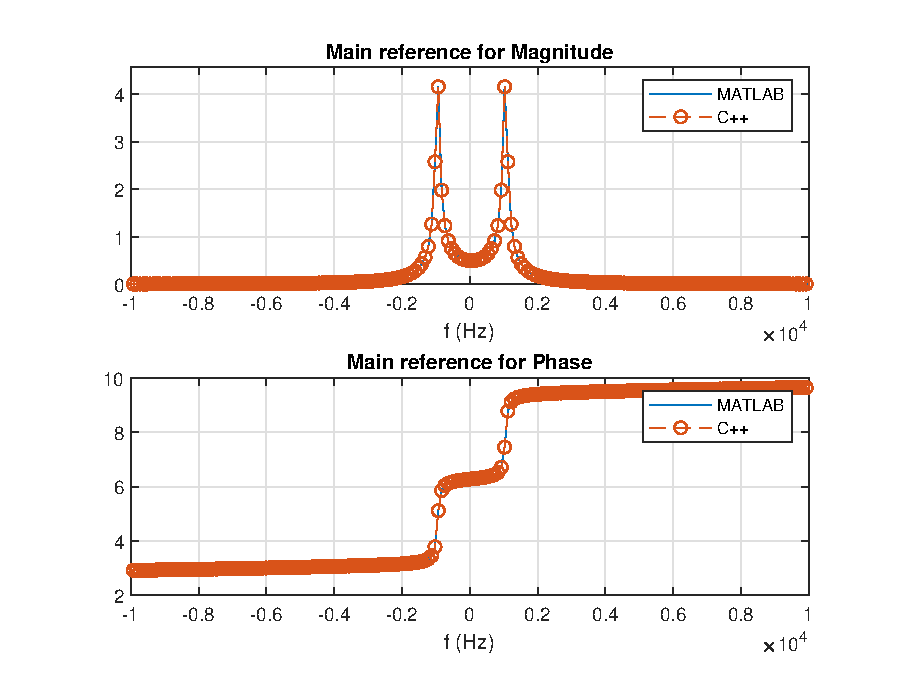
\includegraphics[width=12cm]{./algorithms/fft/figures/Single_sinusoid_fft.eps}
	\caption{MATLAB and C++ comparison}\label{Single_sinusoid_fft}
\end{figure}

\newpage
\subsubsection{3. Mixed signal}

\begin{figure}[h]
	\centering
	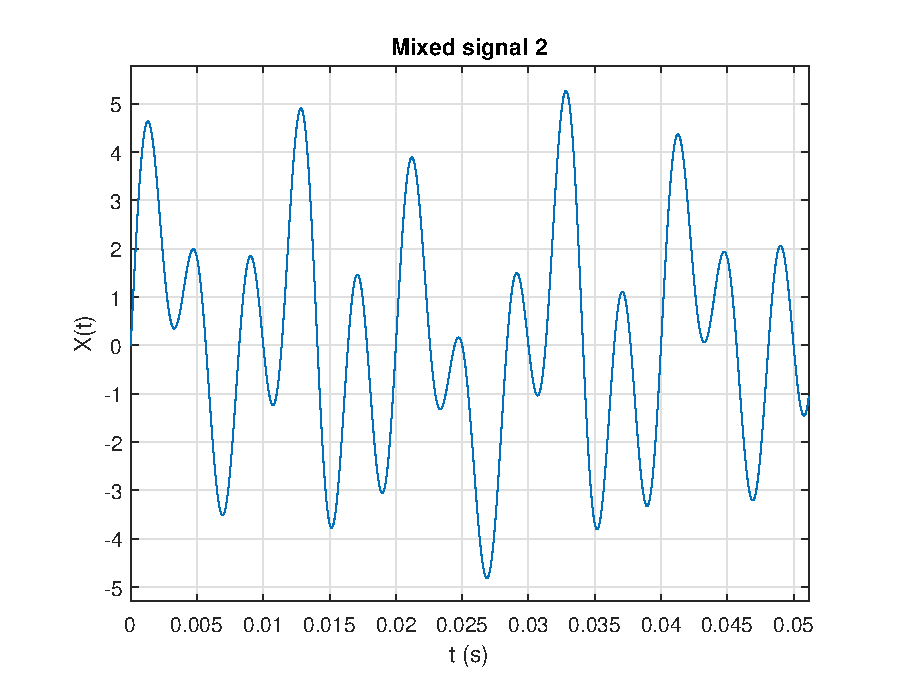
\includegraphics[width=12cm]{./algorithms/fft/figures/mixed_signal.eps}
	\caption{mixed signal}\label{mixed_signal}
\end{figure}

\begin{figure}[h]
	\centering
	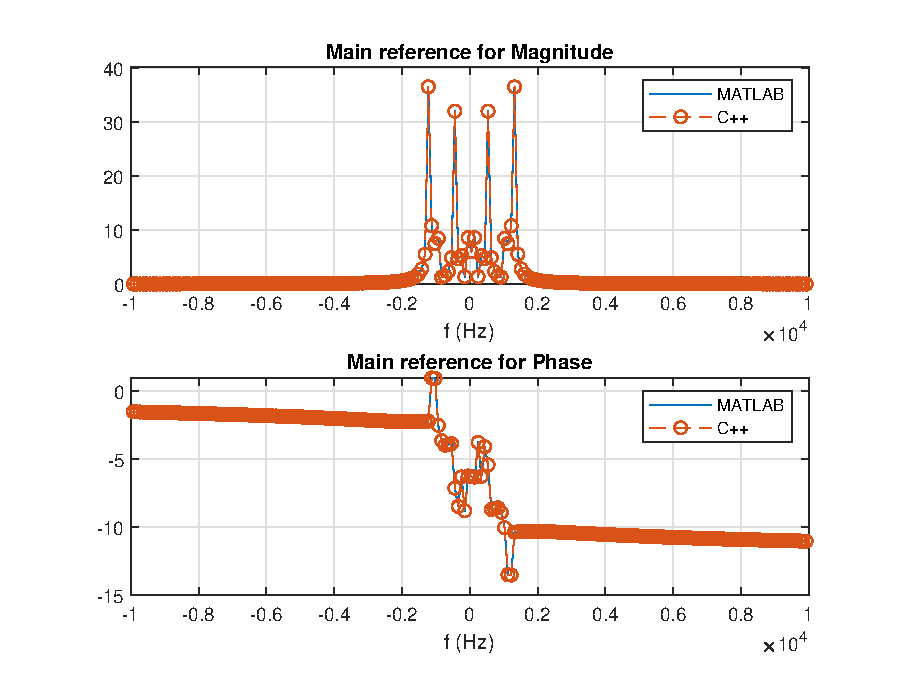
\includegraphics[width=12cm]{./algorithms/fft/figures/mixed_signal_fft.eps}
	\caption{MATLAB and C++ comparison}\label{mixed_signal_fft}
\end{figure}
\subsection*{Remarks}
To write the data from the MATLAB in the form of text file, \textbf{fprintf} MATLAB function was used with the accuracy of the 15 digits. Similarly; to write the fft calculated data from the C++ in the form of text file, C++ \textbf{double} data type with precision of 15 digits applied to the object of \textbf{ofstream} class.\
\section*{Optimized FFT}
\subsubsection{Algorithm}
The algorithm for the optimized FFT will be implemented according with the following expression,
\begin{equation}
X_k =\sum\limits_{n=0}^{N-1} x_n \hspace{2mm} e^{m\hspace{1mm}i2\pi kn/N}		\hspace{2cm}	0\leq k \leq N-1
\label{optimized_FFT}
\end{equation}
Similarly, for IFFT,
\begin{equation}
x_n =\frac{1}{N} \sum\limits_{k=0}^{N-1} X_k \hspace{2mm}  e^{m\hspace{1mm}i2\pi kn/N}		\hspace{2cm}	0\leq k \leq N-1
\label{optimized_IFFT}
\end{equation}
where, $X_k$ is the Fourier transform of $x_n$, and $m$ equals 1 or -1 for FFT and IFFT, respectively.

\subsubsection{Function description}
To perform optimized FFT operation, the fft\_*.h header file must be included and the input argument to the function can be given as follows,
\begin{equation*}
	y=f\hspace{-0.85mm}ft(x,1,1)
\end{equation*}
where $x$ and $y$ are of the C++ type vector<complex>. In a similar way, IFFT can be manipulated as,
\begin{equation*}
	x=f\hspace{-0.85mm}ft(y,-1,1)
\end{equation*}
If we manipulate the optimized FFT and IFFT functions as $y=f\hspace{-0.85mm}ft(x,1,0)$ and  $x=f\hspace{-0.85mm}ft(y,-1,0)$ then it'll calculate the FFT and IFFT as discussed in equation \ref{FFT} and \ref{IFFT} respectively.
\subsubsection{Comparative analysis }
The following table displays the comparative analysis of time elapsed by FFT and optimized FFT for the various length of the data sequence. This comparison performed on the computer having configuration of 16 GB RAM, i7-3770 CPU @ 3.40GHz with 64-bit Microsoft Windows 10 operating system.
\begin{center}
	\begin{tabular}{ |p{4cm}||p{3cm}|p{3cm}|p{3cm}|   }
		\hline
		\centering \textbf{Length of data} & \textbf{Optimized FFT}& \textbf{FFT}&\textbf{MATLAB}\\
		\hline
		\hline
		\centering \textbf{$2^{10}$}   & 0.011 s  & 0.012 s & 0.000485 s\\
		\hline
		\centering \textbf{$2^{10}+1$} & 0.174 s  & 0.179 s & 0.000839 s\\
		\hline
		\centering \textbf{$2^{15}$}   & 0.46 s   & 0.56 s  & 0.003470 s\\
		\hline
		\centering \textbf{$2^{15}+1$} & 6.575 s  & 6.839 s & 0.004882 s\\
		\hline
		\centering \textbf{$2^{18}$}   & 4.062 s  & 4.2729 s& 0.016629 s \\
		\hline
		\centering \textbf{$2^{18}+1$} & 60.916 s & 63.024 s& 0.018992 s\\
		\hline
		\centering \textbf{$2^{20}$}   & 18.246 s & 19.226 s&  0.04217 s\\
		\hline
		\centering \textbf{$2^{20}+1$} & 267.932 s & 275.642 s & 0.04217 s \\
		\hline
	\end{tabular}
\end{center}




% bibliographic references for the section ----------------------------
\clearpage
\printbibliography[heading=subbibliography]
\end{refsection}
\addcontentsline{toc}{subsection}{Bibliography}
\cleardoublepage
% --------------------------------------------------------------------- 


